% ====================================================================
%  Background (~5 min) -- definitions used throughout the talk
%  Layout: text/maths left and figure right; wide thesis figures go
%  full width at the bottom with the definition above them.
% ====================================================================

\begin{frame}{The individual survival distribution (ISD)}
\begin{columns}[c]
  \begin{column}{0.64\textwidth}
    \small
    \textbf{Survival function} for covariates $\bm{x}$:
    \[
      S_E(t \mid \bm{x}) = \Pr(E > t \mid X = \bm{x}) = 1 - F_E(t \mid \bm{x})
    \]
    From one curve we can read off
    \begin{itemize}
      \item a risk ranking,
      \item a probability, e.g.\ $S_E(1 \mid \bm{x}_i) = 0.70$ ({\color{structure.fg}$\bullet$}),
      \item a time, e.g.\ the median $\hat e_i = S_E^{-1}(0.5 \mid \bm{x}_i)$ ({\color{structure.fg}$\blacktriangledown$}),
      \item or the mean $\int_0^\infty S_E(t \mid \bm{x}_i)\, \d t$.
    \end{itemize}
    \vspace{0.3em}
    \textbf{Population baseline} \cite{kaplan_nonparametric_1958}:
    \[
      \hat S_{\text{KM}}(t) = \prod_{j:\, t_j \le t} \Big(1 - \frac{d_j}{n_j}\Big)
    \]
  \end{column}
  \begin{column}{0.34\textwidth}
    \centering
    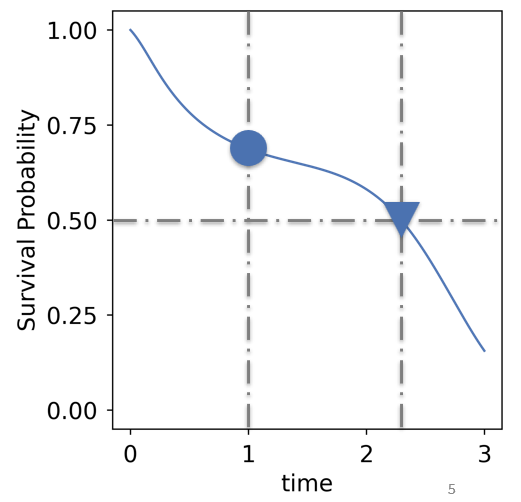
\includegraphics[width=\linewidth]{survival_isd.png}
    \figsource{Figure courtesy of Qi et al.~\cite{qi2025enhancing}}
  \end{column}
\end{columns}
\end{frame}

\begin{frame}{Censoring assumptions matter}
\small
\begin{columns}[T]
  \begin{column}{0.32\textwidth}
    \textbf{Random:} $C \perp (E, X)$
  \end{column}
  \begin{column}{0.32\textwidth}
    \textbf{Independent:} $E \perp C \mid X$
  \end{column}
  \begin{column}{0.32\textwidth}
    \textbf{Dependent:} $E \not\perp C \mid X$
  \end{column}
\end{columns}
\vspace{0.4em}
Under independent censoring the likelihood factorizes and the censoring distribution drops out:
\[
  \mathcal{L}(\bm{\theta}) = \prod_{i=1}^{N}
  f_E(t_i \mid \bm{x}_i)^{\delta_i}\, S_E(t_i \mid \bm{x}_i)^{1-\delta_i}
\]
\vspace{-0.4em}
Under dependent censoring it does not: we need the \emph{joint} law of $(E, C)$.
\vspace{0.2em}
\begin{center}
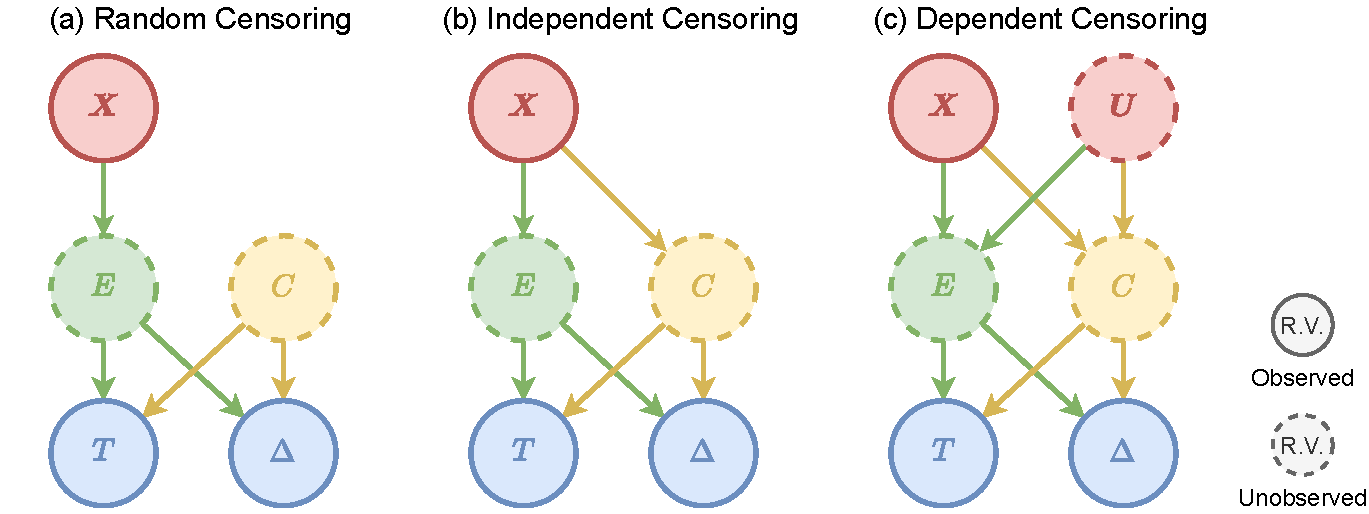
\includegraphics[width=0.72\linewidth]{censoring_assumptions.pdf}
\end{center}
\vspace{-0.6em}
\figsource{Figure courtesy of Qi et al.~\cite{qi_current_2025}}
\end{frame}

\begin{frame}{Two models used throughout: CoxPH and Weibull}
\small
\setlength{\abovedisplayskip}{4pt}\setlength{\belowdisplayskip}{4pt}
\setlength{\abovedisplayshortskip}{3pt}\setlength{\belowdisplayshortskip}{3pt}
The \textbf{hazard} $h(t \mid \bm{x})$ is the event rate at time $t$ among those still event-free.
Both models split it into a shared part and a personal part:
\[
  h(t \mid \bm{x}) \;=\; \underbrace{h_0(t)}_{\text{baseline, shared}} \;\cdot\; \underbrace{\exp(\bm{\beta}^\top \bm{x})}_{\text{personal risk score}}
\]
\vspace{0.3em}
\begin{columns}[T]
  \begin{column}{0.49\textwidth}
    \textbf{CoxPH} \cite{cox_regression_1972}
    \begin{itemize}
      \item Makes \emph{no} assumption about the shape of $h_0(t)$
      \item Learns only $\bm{\beta}$
      \item $e^{\beta_j}$ = \textbf{hazard ratio}: one unit more of $x_j$ multiplies the risk by $e^{\beta_j}$
      \item Widely used and easy to interpret
    \end{itemize}
  \end{column}
  \begin{column}{0.49\textwidth}
    \textbf{Weibull}
    \begin{itemize}
      \item Assumes $h_0(t) \propto t^{\phi}$: the risk rises, stays flat or falls over time
      \item Learns $\bm{\beta}$ and the shape $\phi$
      \item Smooth survival curve in closed form
    \end{itemize}
    \vspace{0.3em}
    \centering
    \begin{tikzpicture}[x=1.0cm,y=0.5cm,font=\scriptsize]
      \draw[->] (0,0) -- (3.0,0) node[below] {$t$};
      \draw[->] (0,0) -- (0,2.5) node[above] {$h_0(t)$};
      \draw[thick,structure.fg] plot[domain=0:2.8,samples=50] (\x,{0.28*\x*\x}) node[right] {$\phi > 0$};
      \draw[thick,black!60] (0,1) -- (2.8,1) node[right] {$\phi = 0$};
      \draw[thick,red!70!black] plot[domain=0.14:2.8,samples=50] (\x,{0.75/sqrt(\x)}) node[right] {$\phi < 0$};
    \end{tikzpicture}
  \end{column}
\end{columns}
\vspace{0.3em}
\takeaway{Same shape over time for everyone -- the risk score $\bm{\beta}^\top \bm{x}$ alone ranks individuals.}
\end{frame}

\begin{frame}{Evaluating survival models: three families of metrics}
\small
\setlength{\abovedisplayskip}{3pt}\setlength{\belowdisplayskip}{3pt}
\setlength{\abovedisplayshortskip}{3pt}\setlength{\belowdisplayshortskip}{3pt}
\begin{columns}[c]
  \begin{column}{0.6\textwidth}
    \textbf{Discrimination} -- is the ranking right? \cite{harrell1996multivariable}
    \[
      \text{CI} = \frac{\sum_{i,j} \delta_i \, \mathbbm{1}[t_i < t_j] \, \mathbbm{1}[\hat\eta_i > \hat\eta_j]}
                       {\sum_{i,j} \delta_i \, \mathbbm{1}[t_i < t_j]}
    \]
    {\footnotesize Share of comparable pairs ranked correctly.\par}
  \end{column}
  \begin{column}{0.38\textwidth}
    \centering
    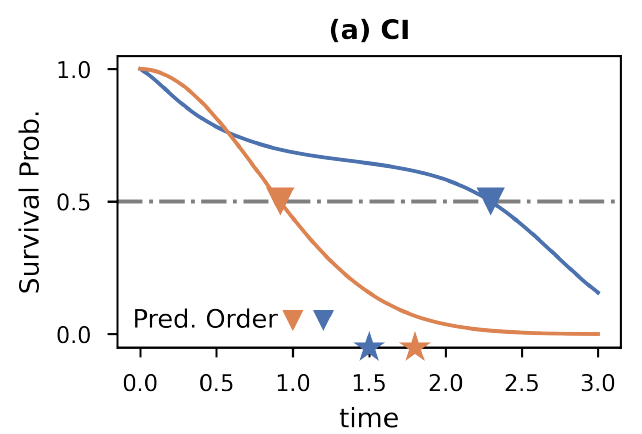
\includegraphics[height=0.25\textheight]{metric_ci.png}
  \end{column}
\end{columns}
\vspace{0.5em}
\begin{columns}[c]
  \begin{column}{0.56\textwidth}
    \textbf{Error} -- how far off are the predictions? \cite{qi2023effective, graf1999assessment}\\
    {\footnotesize Absolute error in time, squared error in probability:}
    {\footnotesize
    \begin{align*}
      \text{MAE} &= \tfrac{1}{N}\textstyle\sum_{i} |e_i - \hat e_i| \\
      \text{IBS} &= \tfrac{1}{t_{\max}}\textstyle\int_0^{t_{\max}} \tfrac{1}{N}\sum_{i} \big(\mathbbm{1}[e_i > t] - \hat S(t \mid \bm{x}_i)\big)^2 \d t
    \end{align*}
    \par}
  \end{column}
  \begin{column}{0.42\textwidth}
    \centering
    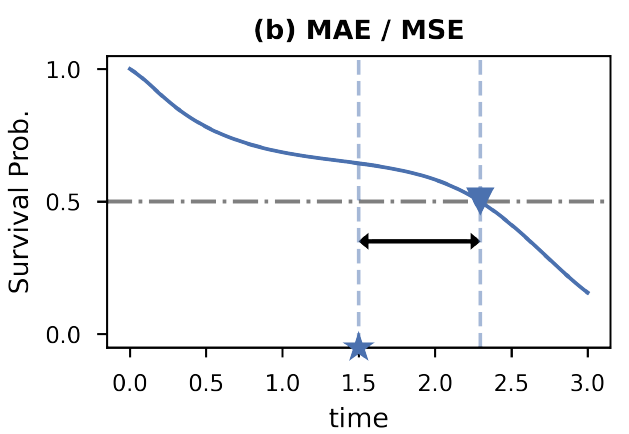
\includegraphics[width=0.49\linewidth]{metric_mae.png}\hfill
    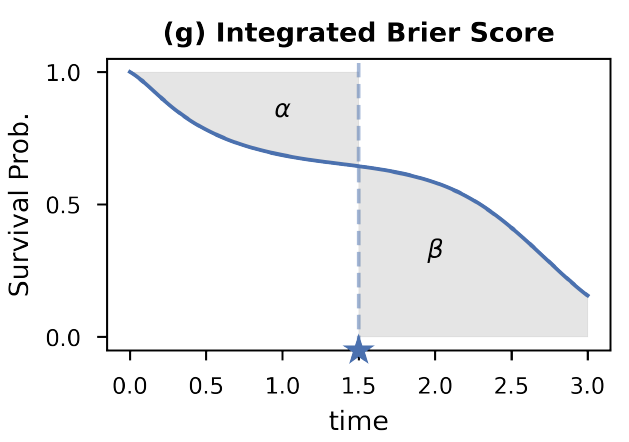
\includegraphics[width=0.49\linewidth]{metric_ibs.png}
  \end{column}
\end{columns}
\vspace{0.5em}
\begin{columns}[c]
  \begin{column}{0.6\textwidth}
    \textbf{Calibration} -- are the probabilities right? \cite{haider2020effective}
    \[
      \hat S(e_i \mid \bm{x}_i) \sim \mathcal{U}(0, 1)
    \]
    {\footnotesize D-calibration: read each curve at its true event time; the values should be uniform.\par}
  \end{column}
  \begin{column}{0.38\textwidth}
    \centering
    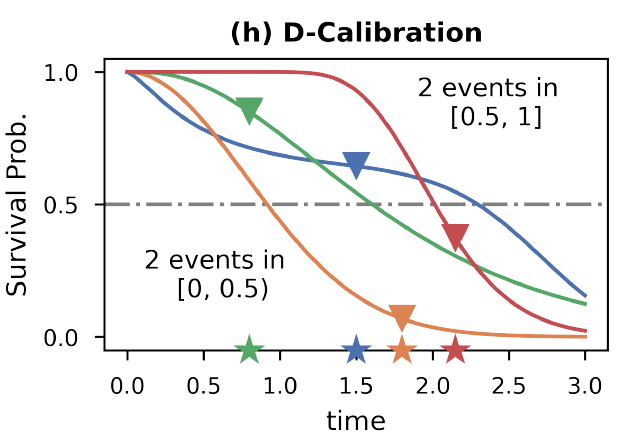
\includegraphics[height=0.25\textheight]{metric_dcal.png}
  \end{column}
\end{columns}
\figsource{Figures courtesy of Qi et al.~\cite{qi_current_2025}}
\end{frame}

\begin{frame}{One event, competing risks, or multiple events}
\begin{columns}[c]
  \begin{column}{0.58\textwidth}
    \small
    \textbf{Single event}: one transition, e.g.\ alive $\to$ dead: $S(t \mid \bm{x})$.\\[0.4em]
    \textbf{Competing risks}: only the \emph{first} of $K$ events is observed: $T = \min_k E_k$.\\[0.4em]
    \textbf{Multiple events}: all $K$ events can occur, in any order: $(t_k, \delta_k)$ for $k = 1, \dots, K$.
  \end{column}
  \begin{column}{0.4\textwidth}
    \centering
    {\footnotesize\textbf{Single event}}\\[0.3em]
    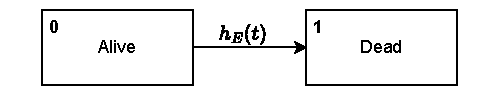
\includegraphics[width=0.8\linewidth]{single_event_model.pdf}
  \end{column}
\end{columns}
\vspace{0.6em}
\begin{columns}[b]
  \begin{column}{0.48\textwidth}
    \centering
    {\footnotesize\textbf{Competing risks}}\\[0.3em]
    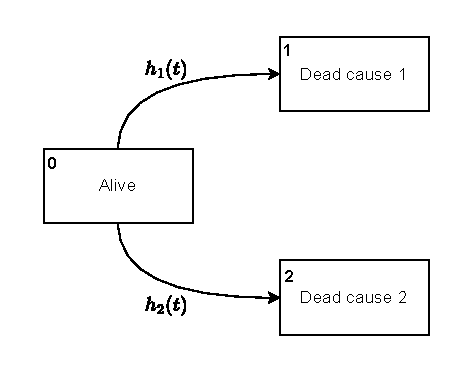
\includegraphics[height=0.31\textheight,width=0.85\linewidth,keepaspectratio]{competing_risks_model.pdf}
  \end{column}
  \begin{column}{0.48\textwidth}
    \centering
    {\footnotesize\textbf{Multiple events}}\\[0.3em]
    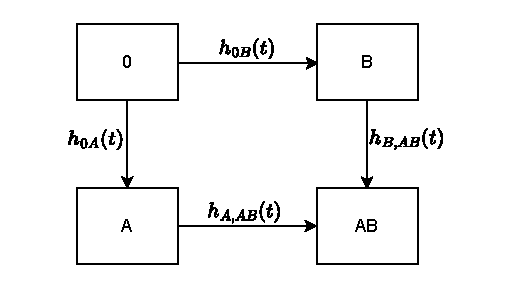
\includegraphics[height=0.31\textheight,width=0.85\linewidth,keepaspectratio]{multi_event_model.pdf}
  \end{column}
\end{columns}
\figsource{Figures from Lillelund et al.~\cite{lillelund_mensa_2026}}
\end{frame}
